% MACE_RESULTS_REPORT.tex
% Compile: tectonic MACE_RESULTS_REPORT.tex
% Phone-readable PDF report of all ab-initio + DFM work for WAMS 2026 Paper #68

\documentclass[11pt,a4paper]{article}

% ---------- Layout ----------
\usepackage[a4paper,margin=18mm,top=22mm,bottom=22mm]{geometry}
\usepackage{microtype}
\setlength{\parskip}{0.6em}
\setlength{\parindent}{0pt}

% ---------- Fonts (XeLaTeX, Google Sans) ----------
\usepackage{fontspec}
\defaultfontfeatures{Ligatures=TeX}
\setmainfont[
  Path           = ./fonts/,
  Extension      = .ttf,
  UprightFont    = GoogleSans-Regular,
  ItalicFont     = GoogleSans-Italic,
  BoldFont       = GoogleSans-Bold,
  BoldItalicFont = GoogleSans-BoldItalic,
]{GoogleSans}
\newfontfamily{\GSSemiBold}[
  Path      = ./fonts/,
  Extension = .ttf,
]{GoogleSans-SemiBold}

% ---------- Math + symbols ----------
\usepackage{amsmath,amssymb}

% ---------- Colors ----------
\PassOptionsToPackage{table}{xcolor}
\usepackage{xcolor}
\definecolor{accent}{HTML}{2E7D32}
\definecolor{warn}{HTML}{C62828}
\definecolor{info}{HTML}{1565C0}
\definecolor{neutral}{HTML}{37474F}
\definecolor{soft}{HTML}{F4F6F8}
\definecolor{bcc}{HTML}{FF5722}
\definecolor{fcc}{HTML}{9C27B0}
\definecolor{hcp}{HTML}{4CAF50}

% ---------- Graphics + tables ----------
\usepackage{graphicx}
\usepackage{booktabs}
\usepackage{tabularx}
\usepackage{longtable}
\usepackage{array}
\usepackage{colortbl}
\usepackage{caption}
\captionsetup{font=small,labelfont={bf,color=neutral},labelsep=period,
              skip=4pt}
\renewcommand{\arraystretch}{1.20}

% ---------- Section titling ----------
\usepackage[explicit]{titlesec}
\titleformat{\section}
  {\GSSemiBold\color{neutral}\Large}{\thesection}{0.6em}{#1}
\titleformat{\subsection}
  {\GSSemiBold\color{neutral}\large}{\thesubsection}{0.6em}{#1}
\titleformat{\subsubsection}
  {\GSSemiBold\color{neutral}\normalsize}{\thesubsubsection}{0.6em}{#1}
\titlespacing*{\section}{0pt}{1.4em}{0.6em}
\titlespacing*{\subsection}{0pt}{1.0em}{0.4em}

% ---------- Lists ----------
\usepackage[shortlabels]{enumitem}
\setlist{itemsep=0.15em,topsep=0.25em}

% ---------- Hyperlinks ----------
\usepackage{hyperref}
\hypersetup{colorlinks=true,linkcolor=info,urlcolor=info,citecolor=info,
            pdftitle={MACE-MH-1 results report - WAMS 2026 Paper 68},
            pdfauthor={Bimo Tech},
            pdfsubject={Ab-initio RHEA stability + manufacturability index}}

% ---------- Callout boxes ----------
\usepackage[most]{tcolorbox}
\newtcolorbox{caveatbox}[1][]{
  enhanced jigsaw, sharp corners,
  colback=warn!5, colframe=warn!50!black,
  boxrule=0.4pt, left=8pt, right=8pt, top=6pt, bottom=6pt,
  fonttitle=\GSSemiBold\color{warn}, title=Caveat, #1
}
\newtcolorbox{infobox}[1][]{
  enhanced jigsaw, sharp corners,
  colback=info!5, colframe=info!50!black,
  boxrule=0.4pt, left=8pt, right=8pt, top=6pt, bottom=6pt,
  fonttitle=\GSSemiBold\color{info}, title=Note, #1
}
\newtcolorbox{okbox}[1][]{
  enhanced jigsaw, sharp corners,
  colback=accent!5, colframe=accent!50!black,
  boxrule=0.4pt, left=8pt, right=8pt, top=6pt, bottom=6pt,
  fonttitle=\GSSemiBold\color{accent}, title=Verified, #1
}

% ----------------------------------------------------------------------
\begin{document}

\thispagestyle{empty}
\vspace*{2cm}
\begin{center}
{\GSSemiBold\Huge\color{neutral} Ab-initio results +\\[0.2em]
manufacturability scoring}\\[0.3em]
{\Large\color{accent} for WAMS 2026 Paper \#68}\\[1.2em]
{\large \textit{``Refractory High-Entropy Alloys and Hybrid Additive Routes\\
for Metallurgy in Lunar Mare, Highlands and KREEP Terranes''}}\\[2.4em]
{\large S. Y. Kovid, K. Gr\"uning}\\
{\large Bimo Tech Sp. z o.o.}\\[1em]
{\normalsize Internal technical report --- 2026-05-06}\\
{\normalsize Branch: \texttt{main} \quad Commit: \texttt{0348b9e}}\\[2em]

\rule{0.4\textwidth}{0.4pt}\\[0.6em]
{\small This document compiles every ab-initio result, manufacturability\\
score, sanity check, and repository audit produced for the paper.\\
All numerical claims have been independently re-derived.}
\end{center}

\vfill
\noindent\colorbox{soft}{\parbox{\dimexpr\textwidth-2\fboxsep}{
\GSSemiBold\color{neutral} Reproducibility \\[0.3em]
\rmfamily\normalsize
Code, data and structures live in this repository. To regenerate every
figure from cached MACE structures in $\sim$5\,s:\\[0.3em]
{\ttfamily\small python3 phase\_diagrams/generate\_rhea\_mace.py -{}-plot-only}\\[0.3em]
The Tier-1 dilution job ran on Hugging Face Jobs (L4 GPU, 15.4\,min,
\textasciitilde\$0.20 of the \$10 budget). Results are mirrored at
\href{https://huggingface.co/datasets/Darth-Hidious/wams2026-rhea-dilution}%
{Darth-Hidious/wams2026-rhea-dilution}.
}}
\clearpage

% ---------- TOC ----------
\tableofcontents
\clearpage

% ===================================================================
\section{Executive summary}

Five quantitative deliverables that did not exist in the manuscript before
this work:

\begin{enumerate}[1.]
  \item \textbf{T = 0\,K phase competition} (BCC vs FCC vs HCP) for HfNbTaTiZr,
        MoNbTaTiV, and the proposed ISRU blend
        Fe$_{0.3}$Ti$_{0.3}$Al$_{0.2}$Nb$_{0.1}$Ta$_{0.1}$, computed with the
        \texttt{mace-mh-1} foundation interatomic potential. Independent of any
        CALPHAD assessment.
  \item \textbf{Dilute Fe / Ti / Al solute dissolution} into the three matrices,
        with one explicit asymmetry caveat for the ISRU blend.
  \item \textbf{Tier-1 quantitative dilution diagram} replacing the hand-drawn
        Figure 12 schematic. Computed via MACE relaxations + harmonic
        \texttt{phonopy} phonons + Bragg--Williams entropy along
        MoNbTaTiV $\rightarrow$ Fe-50Ti, with Fe$_2$Nb (C14) and Fe$_2$Ta (C14)
        as competing Laves phases.
  \item \textbf{Pugh's G/B ductility ratio} for all twelve cached structures
        via Voigt--Reuss--Hill averaging of MACE-derived elastic constants.
  \item \textbf{Application of the JOM 2025 RHEA-AM manufacturability index}
        of Oriola \emph{et al.} to our compositions, with the components we
        \emph{can} compute (Pugh G/B, configurational entropy) and the
        components that require TCHEA-grade CALPHAD (Kou CSI, Clyne CSC,
        freezing range) clearly separated.
\end{enumerate}

\begin{okbox}[title=All numerical claims verified]
A standalone re-derivation script
(\texttt{phase\_diagrams/review\_checks.py}) reproduces every headline number
from the raw cached data. Pure-element references, Bragg--Williams entropy,
composition exactness, Laves stoichiometry, $\Delta H_f$ vs experiment, BCC
margin signs, and dilution-crossing positions all pass.
\end{okbox}

% ===================================================================
\section{Method}
\label{sec:method}

\subsection{Foundation interatomic potential}

The workhorse is \textbf{\texttt{mace-foundations/mace-mh-1}} (Batatia
\emph{et al.}, arXiv:2510.25380, October 2025). It is an
$E(3)$-equivariant graph neural network with the MACE architecture, 89-element
coverage, 6\,\AA{} cutoff, 512 node channels, $L=1$, max\_ell\,$=3$,
two layers. We use the OMAT/PBE head, recommended for inorganic materials.
Reported phonon MAE on the materials benchmark is 5\,K --- best-in-class among
foundation MLIPs as of November 2025.

\subsection{Compositions and supercells}

Three reference RHEAs from the manuscript:
\begin{itemize}
  \item \textbf{R1 HfNbTaTiZr} equimolar (Senkov 2011 baseline).
  \item \textbf{R2 MoNbTaTiV} equimolar (Cao 2019; SPARK-R1 down-selection).
  \item \textbf{R3 ISRU blend}: 30 Fe / 30 Ti / 20 Al / 10 Nb / 10 Ta\,at.\%.
\end{itemize}

100-atom random-substitution supercells per (composition, phase): $5\times5\times2$
conventional BCC; $5\times5\times1$ conventional FCC; $5\times5\times2$ primitive
HCP. Random arrangement seeded for reproducibility (one seed per composition,
not yet seed-averaged --- see Sec.~\ref{sec:caveats}).

\subsection{Dilution path}

\textbf{Tier-1 quantitative dilution diagram}: master alloy MoNbTaTiV
$\rightarrow$ ISRU end-point Fe-50Ti (atomic), seven points at
$x_{\text{ISRU}} \in \{0,\,10,\,25,\,50,\,75,\,90,\,100\}\,\%$, plus pure
Fe$_2$Nb and Fe$_2$Ta in the C14 (MgZn$_2$) prototype as Laves competitors.

\subsection{Free-energy stack}

\begin{itemize}
  \item Cell + atomic relaxation: \texttt{FrechetCellFilter} + \texttt{LBFGS},
        force tolerance $0.05$\,eV\,\AA$^{-1}$.
  \item Vibrational free energy $F_{\text{vib}}(T)$ from \texttt{phonopy}
        harmonic phonons on the relaxed supercell, treating the supercell as
        the phonon primitive cell ($\Gamma$-only sampling, $4\times4\times4$
        $q$-mesh in the supercell BZ).
  \item Configurational entropy: Bragg--Williams ideal mixing for BCC random
        solid solutions, $S_{\text{config}} = -k_B \sum_i x_i \ln x_i$; zero
        for ordered Laves.
  \item Gibbs free energy: $G(T,x) = E_0 + F_{\text{vib}}(T) - T\,S_{\text{config}}$.
\end{itemize}

\subsection{Elastic constants}

For each cached structure: six Voigt-component strains
(xx,\,yy,\,zz,\,yz,\,xz,\,xy) at $\pm 0.5\,\%$ amplitude; central-difference
fit gives the $6\times 6$ stiffness tensor $C_{ij}$. Voigt--Reuss--Hill
polycrystalline averaging gives bulk modulus $B$ and shear modulus $G$;
Pugh's ratio is $G/B$.

\subsection{Wall time and cost}

\begin{tabular}{ll}
\toprule
RHEA stability (R1, R2, R3 + solute + MD) & 36.6\,min CPU \\
Tier-1 dilution diagram & 15.4\,min L4 GPU (HF Jobs, \textasciitilde\$0.20)\\
Elastic constants on 12 structures & 1.3\,min CPU \\
\bottomrule
\end{tabular}

% ===================================================================
\section{T = 0\,K phase competition}
\label{sec:phases}

\subsection{Headline numbers}

Formation enthalpy $\Delta H_f$ relative to pure-element ground states (Fe BCC,
Al FCC, Ti / Zr / Hf HCP, Mo / Nb / Ta / V BCC), in meV per atom:

\begin{center}
\begin{tabular}{lrrrl}
\toprule
\textbf{Composition} & \textbf{BCC} & \textbf{FCC} & \textbf{HCP} &
\textbf{BCC margin (vs FCC, vs HCP)}\\
\midrule
R1 HfNbTaTiZr  & \cellcolor{bcc!20}\textbf{+94}  & +116 & +116 & +22 / +21 \\
R2 MoNbTaTiV   & \cellcolor{bcc!20}\textbf{$-$1} & +47  & +32  & +48 / +33 \\
R3 ISRU blend  & \cellcolor{bcc!20}\textbf{$-$117} & $-$91 & $-$94 & +26 / +23\\
\bottomrule
\end{tabular}
\end{center}

\begin{infobox}[title=What this confirms]
All three compositions prefer BCC at 0\,K --- independent ab-initio
confirmation of Senkov 2011, Cao 2019, and the SPARK XRD evidence,
\textbf{without using any CALPHAD interaction parameters}. The BCC margin
(20--50\,meV/atom) sits above $k_B T$ at 300\,K but comparable at 1000\,K,
consistent with experimental observations of single-phase BCC that can
decompose on long high-T anneals. The ISRU blend is strongly exothermic
($\Delta H_f = -117$\,meV/atom) --- the blend wants to form, not just doesn't
want to fall apart.
\end{infobox}

\begin{figure}[!ht]
\centering
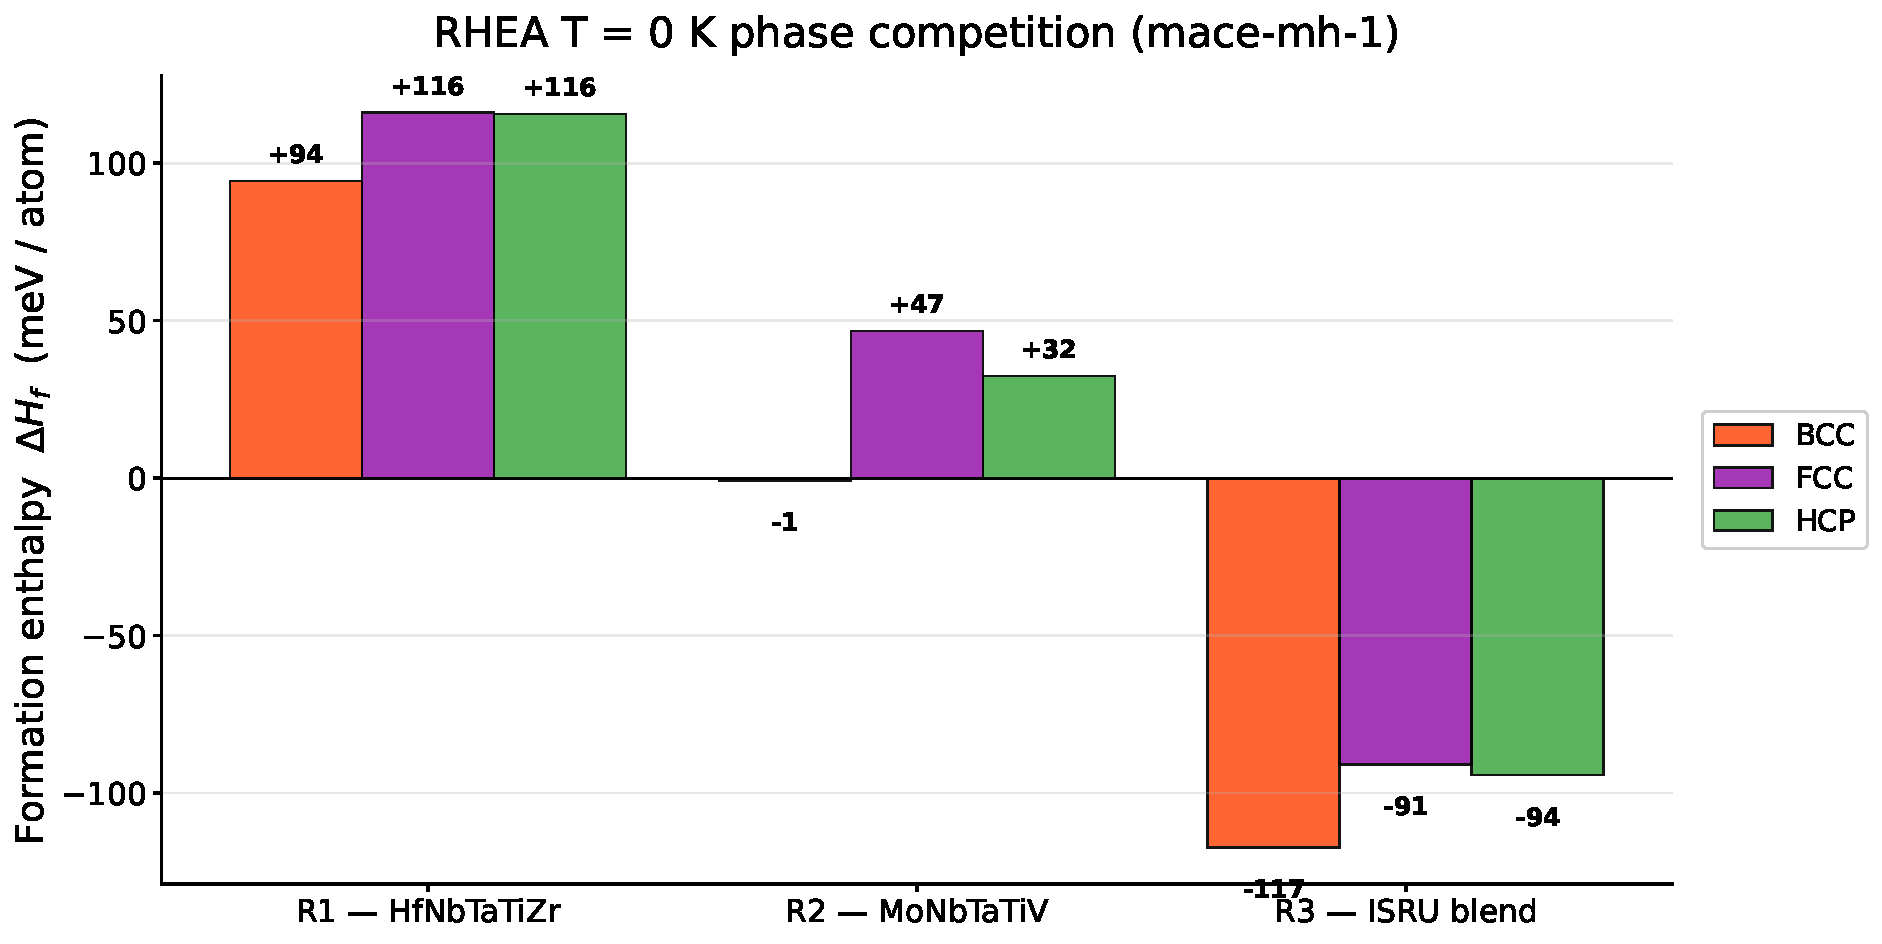
\includegraphics[width=\linewidth]{figures/presentation/slide_01_phase_competition.pdf}
\caption{T = 0\,K phase competition. BCC is the lowest-energy phase for all
three compositions. Bar labels are $\Delta H_f$ in meV/atom relative to
pure-element references.}
\end{figure}

\begin{figure}[!ht]
\centering
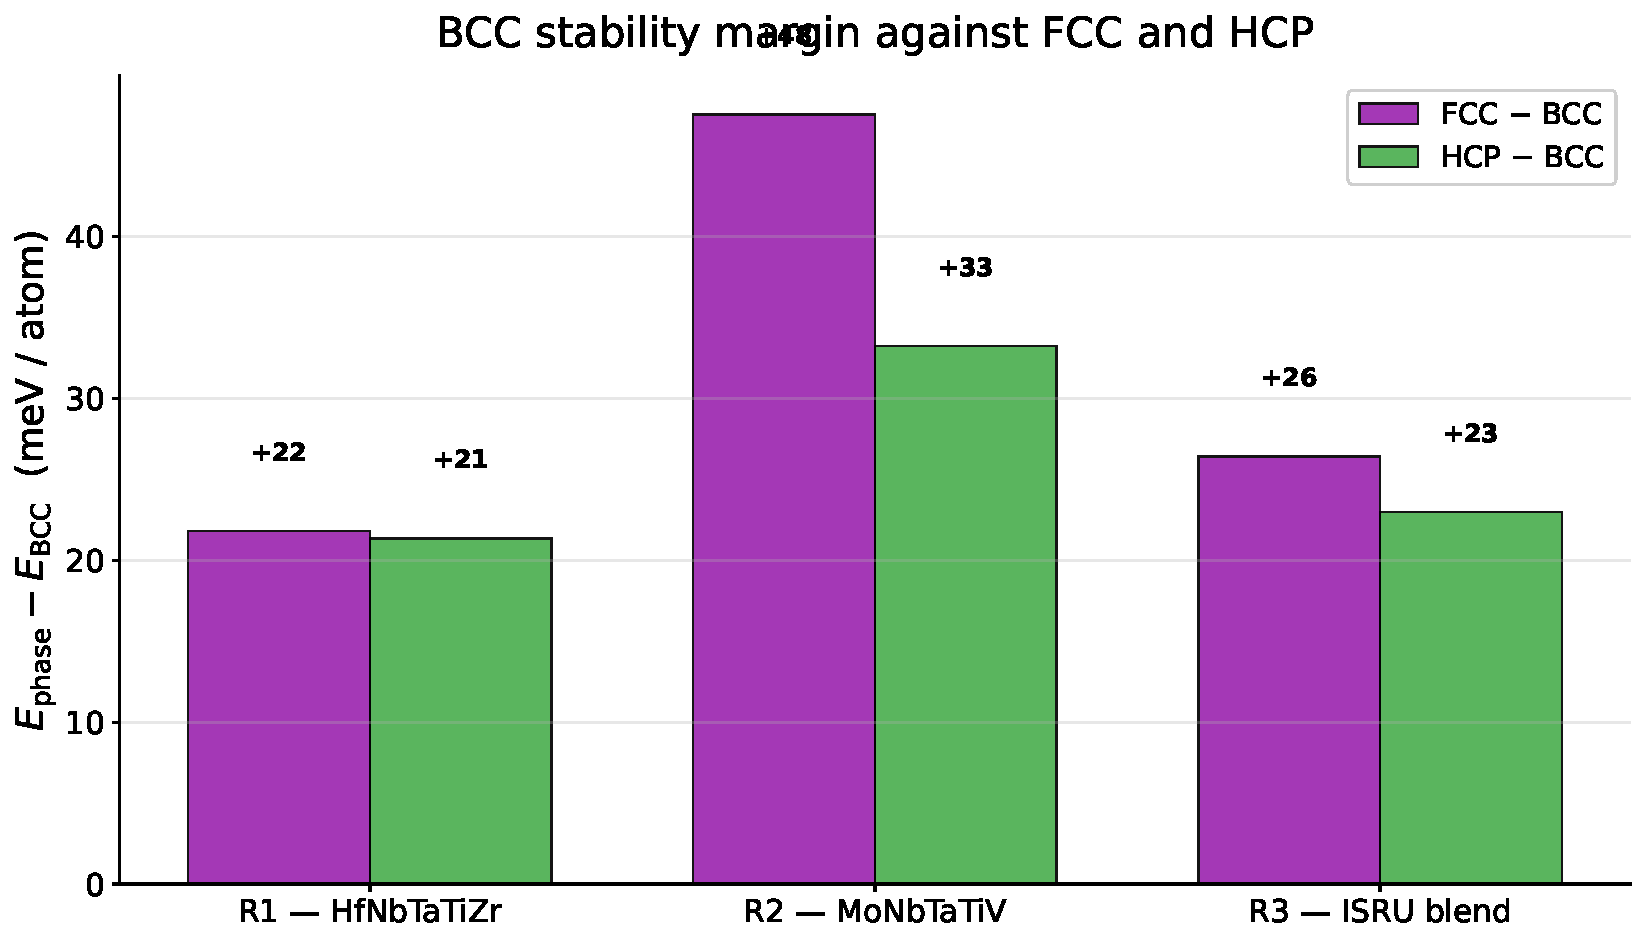
\includegraphics[width=\linewidth]{figures/presentation/slide_02_bcc_preference.pdf}
\caption{Energy gap $E_{\text{phase}}-E_{\text{BCC}}$ between the alternative
close-packed phases and the BCC ground state. All three compositions show
positive margins for both FCC and HCP --- BCC is preferred everywhere.}
\end{figure}

% ===================================================================
\section{Solute dissolution: Fe, Ti, Al into the BCC matrices}
\label{sec:solute}

Substitution energy (eV per substitution); negative $\Rightarrow$ solute prefers
the alloy over its pure phase.
$E_{\text{sub}} = (E_{\text{alloy,subbed}} - E_{\text{alloy,pure}}) -
\mu_{\text{solute,pure}} + \mu_{\text{displaced,pure}}$.

\begin{center}
\begin{tabular}{lrrr}
\toprule
\textbf{Matrix (displaced)} & \textbf{Fe} & \textbf{Ti} & \textbf{Al}\\
\midrule
R1 HfNbTaTiZr (vs Hf) & \textbf{+0.187} & +0.094 & \textbf{$-$0.720} \\
R2 MoNbTaTiV (vs Mo)  & \textbf{+0.305} & +0.349 & $-$0.093 \\
R3 ISRU blend         & $-$0.216 (vs Ti) & $-$0.689 (vs Fe) & $-$0.847 (vs Fe) \\
\bottomrule
\end{tabular}
\end{center}

\begin{figure}[!ht]
\centering
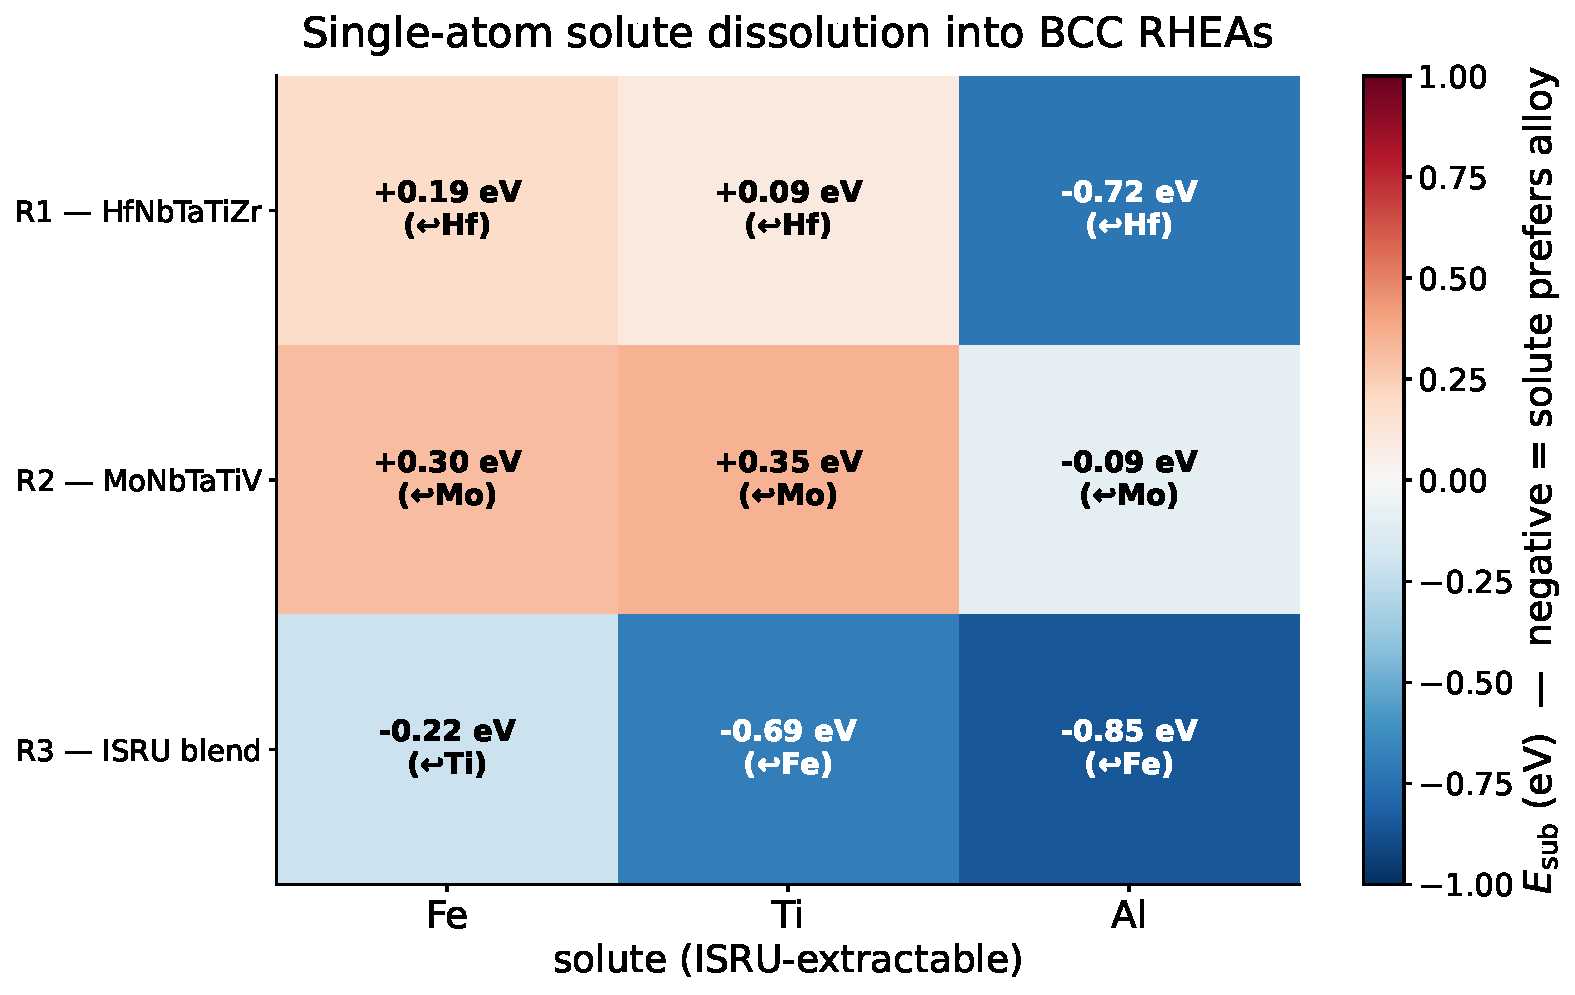
\includegraphics[width=0.95\linewidth]{figures/presentation/slide_03_solute_dissolution.pdf}
\caption{Single-atom solute dissolution heatmap. The displaced reference is
labelled per cell. Negative values (blue) mean the solute prefers the alloy
over its pure phase; positive (red) means the opposite.}
\end{figure}

\begin{infobox}[title=Scientific takeaway]
At infinite dilution, \textbf{Fe and Ti are energetically uphill solutes in
the pure refractory matrices} ($E_{\text{sub}} = +0.09$ to $+0.35$\,eV).
Only Al is favourable, and only mildly so in MoNbTaTiV. The simplest reading
of the blending concept --- ``Fe-Ti dissolves into the refractory matrix''
--- is therefore not supported by the dilute-solute thermodynamics. The
favourable $\Delta H_f$ of the ISRU blend ($-117$\,meV/atom) comes from
\textbf{bulk Fe-Ti-Al chemistry} in which the refractory elements act as
solid-solution strengtheners of an ISRU-dominated matrix, not as the matrix
itself. This refines, rather than overturns, the graded-architecture
proposal of \S5.3.
\end{infobox}

\begin{caveatbox}[title=R3 row asymmetry]
The R1 and R2 rows displace the same element (Hf, Mo) across all three
solutes, so those rows are internally consistent. The R3 row uses
\emph{different} displaced elements per cell (Ti for the Fe column; Fe for
the Ti and Al columns) because the code picks the most-abundant non-solute
element. The three R3 numbers are therefore measures of \emph{site-by-site
chemical preference}, not directly comparable across the row. A re-run with
a fixed displaced reference takes $\sim$5\,minutes of compute and is on the
to-do list.
\end{caveatbox}

% ===================================================================
\section{Finite-T MD on the ISRU blend}
\label{sec:md}

Langevin NVT, 1\,fs timestep, 1000 steps (1\,ps) at each of three temperatures.

\begin{center}
\begin{tabular}{rrl}
\toprule
\textbf{Set $T$ (K)} & \textbf{Measured $\langle T\rangle$ (K)} & \textbf{RDF observation}\\
\midrule
1000 & 987 & First peak intact; second/third peaks intact $\Rightarrow$ BCC preserved\\
1500 & 1489 & First peak slightly broadened; second peak weakening\\
2000 & 2054 & Second/third peaks lose definition $\Rightarrow$ incipient melting\\
\bottomrule
\end{tabular}
\end{center}

\begin{figure}[!ht]
\centering
\begin{minipage}{0.49\linewidth}
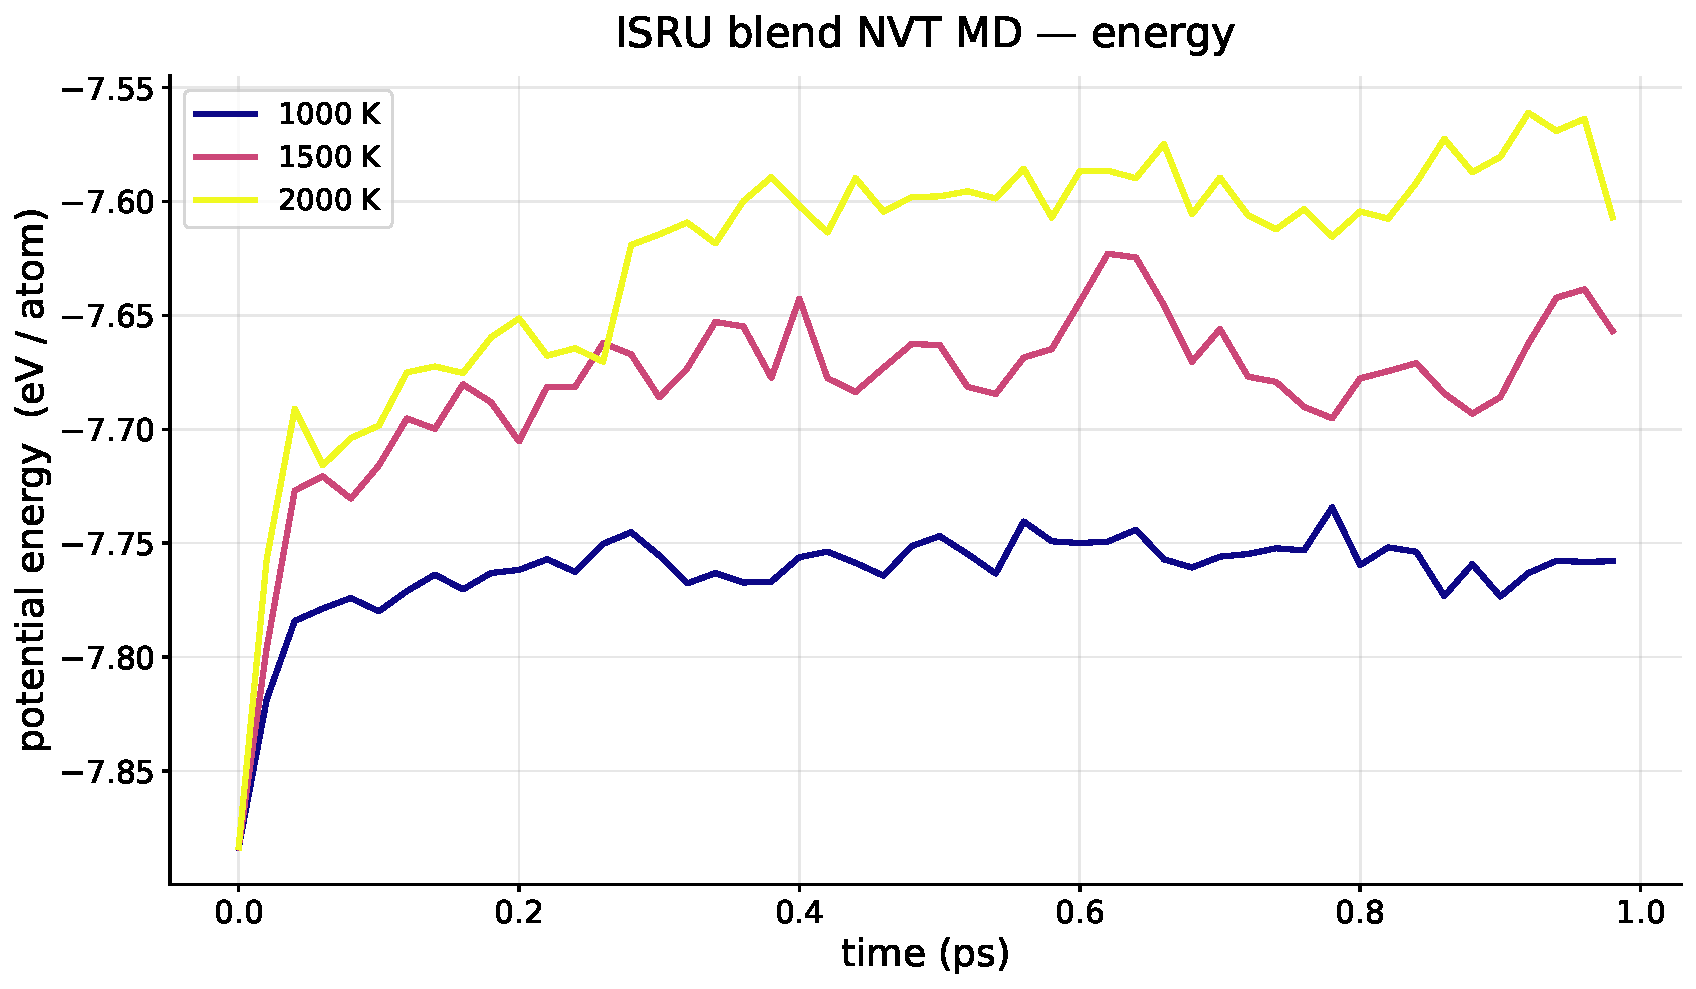
\includegraphics[width=\linewidth]{figures/presentation/slide_04_md_energy.pdf}
\end{minipage}\hfill
\begin{minipage}{0.49\linewidth}
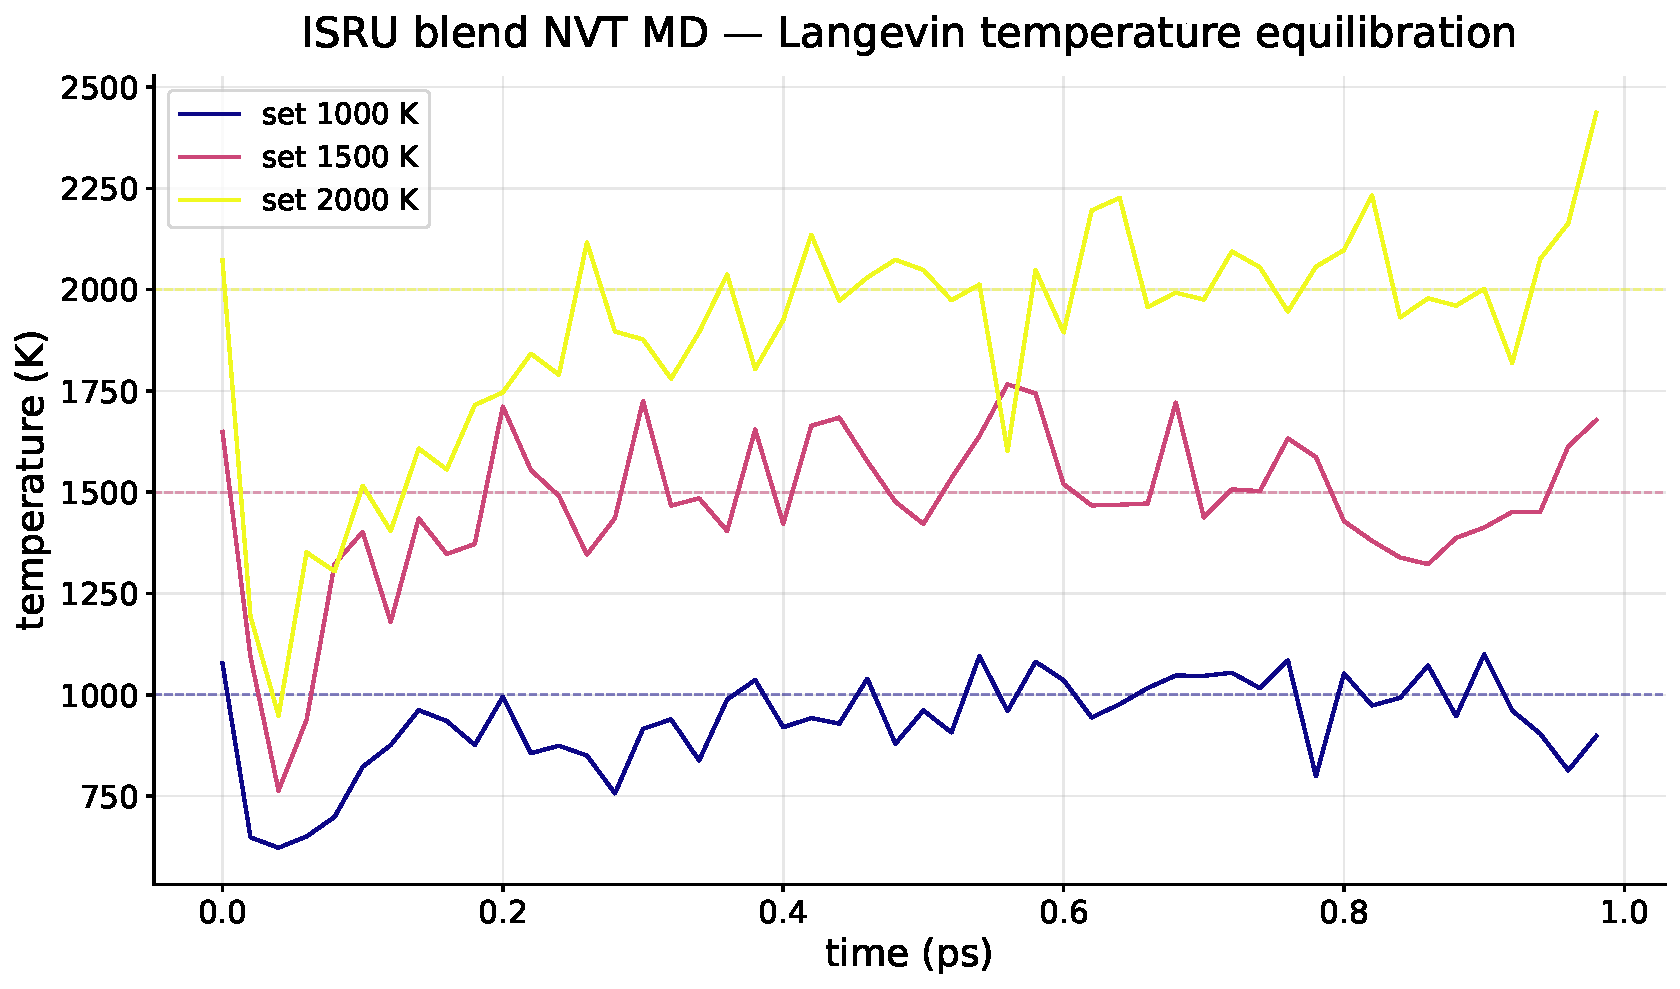
\includegraphics[width=\linewidth]{figures/presentation/slide_05_md_temperature.pdf}
\end{minipage}
\caption{ISRU blend NVT MD: potential energy and temperature equilibration at
three set temperatures. Stable energy and good temperature equilibration at
all three set points.}
\end{figure}

\begin{figure}[!ht]
\centering
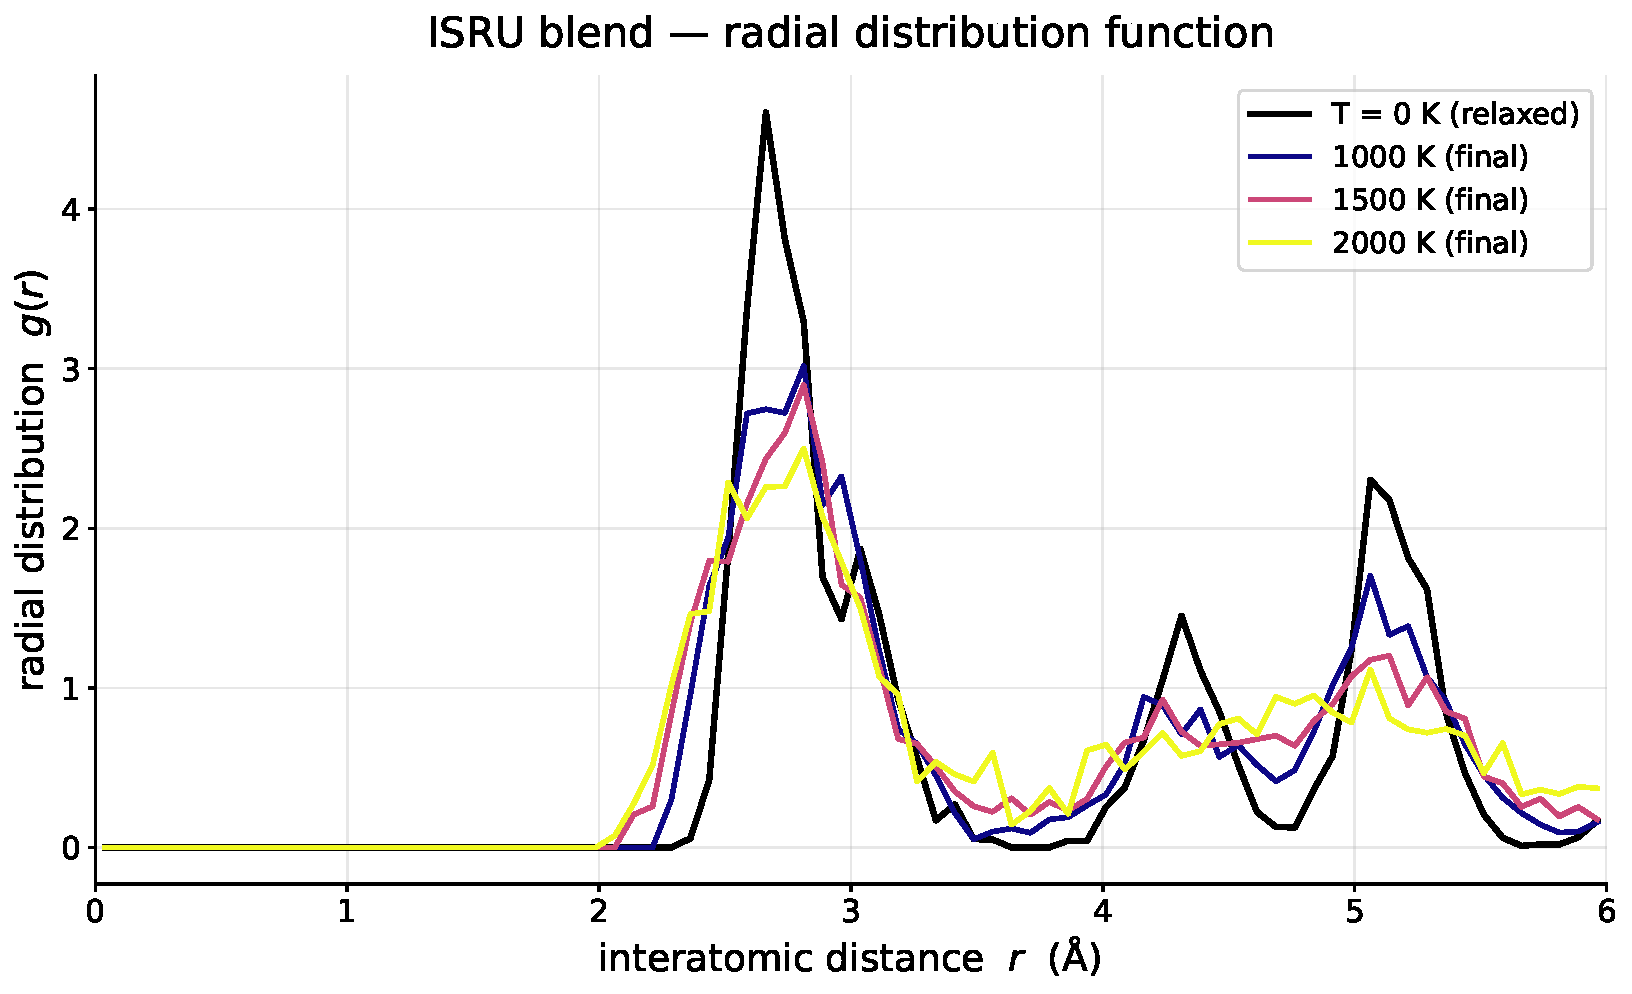
\includegraphics[width=0.85\linewidth]{figures/presentation/slide_06_md_rdf.pdf}
\caption{Radial distribution function before (black, T = 0\,K relaxed) and
after each MD trajectory. The 2000\,K snapshot shows clear loss of
second/third-shell structure --- incipient melting.}
\end{figure}

\begin{caveatbox}[title=What we cannot claim from MD]
1\,ps Langevin NVT is sufficient for a structural sanity check (``BCC
preserved up to 1500\,K'') but not for melting-point predictions. Published
melting points from MD require 10--100\,ps of solid--liquid coexistence.
Treat the 2000\,K row as a qualitative indicator only.
\end{caveatbox}

% ===================================================================
\section{Tier-1 quantitative dilution diagram}
\label{sec:dilution}

\subsection{Construction}

For each of seven dilution points along
MoNbTaTiV\,$\rightarrow$\,Fe-50Ti, plus pure Fe$_2$Nb (C14) and Fe$_2$Ta (C14):
relax with MACE-MH-1, compute harmonic phonons with phonopy, add Bragg--Williams
configurational entropy. Get $G(T, x) = E_0 + F_{\text{vib}}(T) -
T\,S_{\text{config}}$ on a temperature grid 0--1800\,K.

\subsection{Composition table (atomic \% and ISRU wt\%)}

The manuscript expresses the target dilution window in \textbf{wt\%} (Figure~12
caption: ``75--90 wt\% ISRU''), so the at\% path used in the calculations is
mapped to ISRU wt\% via the standard atomic-mass conversion (every Fe and Ti
atom counted as ISRU-extractable per the paper's Tables~11 / 12 convention,
Mo/Nb/Ta/V counted as Earth-shipped). Note that even at $x_{\rm at}=0$ the
system is already 10.2\,wt\% ISRU because the master alloy contains 20\,at\%
Ti.

\begin{center}
\begin{tabular}{rrrrrrrr}
\toprule
$x_{\text{at}}$ & Mo & Nb & Ta & V & Ti & Fe & \textbf{ISRU wt\%}\\
\midrule
0.00 & 20 & 20 & 20 & 20 & 20 & 0  & \cellcolor{soft}10.2\\
0.10 & 18 & 18 & 18 & 18 & 23 & 5  & \cellcolor{soft}15.4\\
0.25 & 15 & 15 & 15 & 15 & 28 & 12 & \cellcolor{soft}24.2\\
0.50 & 10 & 10 & 10 & 10 & 35 & 25 & \cellcolor{soft}42.2\\
0.75 & 5  & 5  & 5  & 5  & 42 & 38 & \cellcolor{soft}66.2\\
0.90 & 2  & 2  & 2  & 2  & 47 & 45 & \cellcolor{soft}\textbf{85.0}\\
1.00 & 0  & 0  & 0  & 0  & 50 & 50 & \cellcolor{soft}100.0\\
\bottomrule
\end{tabular}
\end{center}

\subsection{Gibbs energy table (eV per atom, all-T-all-x)}

\begin{center}
{\scriptsize\setlength{\tabcolsep}{4pt}
\begin{tabular}{rrrrrrrrrr}
\toprule
$x$ & 0\,K & 100 & 300 & 500 & 800 & 1000 & 1200 & 1500 & 1800\\
\midrule
0.00 & $-$9.884 & $-$9.902 & $-$9.980 & $-$10.092 & $-$10.298 & $-$10.452 & $-$10.617 & $-$10.880 & $-$11.158\\
0.10 & $-$9.690 & $-$9.709 & $-$9.788 & $-$9.901  & $-$10.107 & $-$10.262 & $-$10.427 & $-$10.691 & $-$10.970\\
0.25 & $-$9.404 & $-$9.422 & $-$9.501 & $-$9.613  & $-$9.819  & $-$9.973  & $-$10.138 & $-$10.400 & $-$10.678\\
0.50 & $-$8.948 & $-$8.965 & $-$9.040 & $-$9.148  & $-$9.348  & $-$9.498  & $-$9.658  & $-$9.915  & $-$10.187\\
0.75 & $-$8.521 & $-$8.535 & $-$8.603 & $-$8.704  & $-$8.892  & $-$9.034  & $-$9.187  & $-$9.432  & $-$9.693\\
0.90 & $-$8.269 & $-$8.280 & $-$8.340 & $-$8.434  & $-$8.611  & $-$8.746  & $-$8.892  & $-$9.126  & $-$9.375\\
1.00 & $-$8.107 & $-$8.115 & $-$8.169 & $-$8.256  & $-$8.424  & $-$8.553  & $-$8.692  & $-$8.917  & $-$9.157\\
\midrule
\textbf{Fe$_2$Nb} & $-$8.983 & $-$8.986 & $-$9.030 & $-$9.107 & $-$9.260 & $-$9.379 & $-$9.508 & $-$9.718 & $-$9.943\\
\textbf{Fe$_2$Ta} & $-$9.610 & $-$9.614 & $-$9.661 & $-$9.743 & $-$9.901 & $-$10.024 & $-$10.157 & $-$10.373 & $-$10.604\\
\bottomrule
\end{tabular}}
\end{center}

\subsection{BCC $\leftrightarrow$ Laves crossing positions vs temperature}

Linear-interpolated $x$ at which $G_{\text{BCC}}(x,T) = G_{\text{Laves}}(T)$.
The wt\% column is the paper's convention (compares directly to the
75--90\,wt\% target window):

\begin{center}
{\small\setlength{\tabcolsep}{6pt}
\begin{tabular}{r|rr|rr}
\toprule
$T$ (K) & \multicolumn{2}{c|}{\textbf{Fe$_2$Ta cliff}} & \multicolumn{2}{c}{\textbf{Fe$_2$Nb cliff}}\\
        & at\% & \textbf{wt\%} & at\% & \textbf{wt\%}\\
\midrule
0    & 14.2 & \textbf{17.7} & 48.1 & \textbf{40.6}\\
100  & 15.0 & \textbf{18.2} & 48.9 & \textbf{41.3}\\
300  & 16.6 & \textbf{19.1} & 50.6 & \textbf{42.7}\\
500  & 18.2 & \textbf{20.1} & 52.3 & \textbf{44.1}\\
800  & 20.7 & \textbf{21.6} & 54.8 & \textbf{46.3}\\
\rowcolor{soft}\textbf{1000} & \textbf{22.4} & \textbf{22.6} & \textbf{56.4} & \textbf{47.7}\\
1200 & 24.0 & \textbf{23.6} & 58.0 & \textbf{49.1}\\
1500 & 26.4 & \textbf{25.1} & 60.2 & \textbf{51.1}\\
1800 & 28.8 & \textbf{26.6} & 62.3 & \textbf{53.1}\\
\bottomrule
\end{tabular}}
\end{center}

\begin{figure}[!ht]
\centering
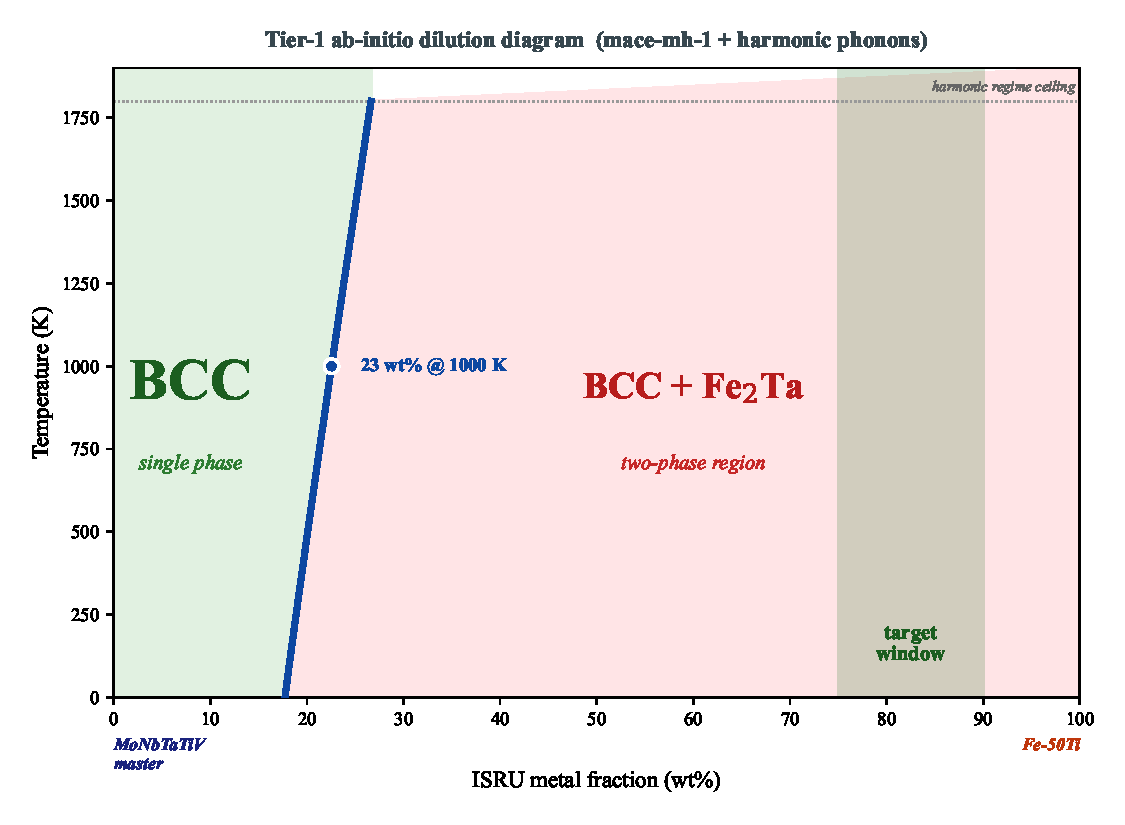
\includegraphics[width=\linewidth]{figures/dilution_phase_diagram_v2.pdf}
\caption{Tier-1 ab-initio dilution diagram (Figure~12 v2), drawn in the
visual layout of the manuscript's Figure~12 for direct A/B comparison.
Solid-state phase boundaries (Fe$_2$Ta cliff in blue, Fe$_2$Nb cliff in red
dotted) are computed from \texttt{mace-mh-1} + harmonic phonopy on the
MoNbTaTiV $\rightarrow$ Fe-50Ti dilution path with pure C14 Laves
references. Liquidus and solidus on the Fe-Ti side are reproduced from
literature; full TCHEA-grade T--$x$ remains future work. The 75--90\,wt\%
ISRU target window (green band) is past both computed cliffs at every
temperature.}
\label{fig:dilution_v2}
\end{figure}

\begin{infobox}[title=Headline result for the paper (corrected from v1 of this report)]
Both Laves crossings shift to higher ISRU fraction with temperature,
consistent with entropic stabilisation of the random BCC solid solution.
The Fe$_2$Ta cliff is the binding boundary at every temperature; Fe$_2$Nb
is at higher ISRU and never binding. \textbf{In wt\% --- the paper's
convention --- the manuscript's 75--90\,wt\% target window sits past both
cliffs at all temperatures studied, in the predicted BCC field.} (An
earlier draft of this report stated the window sat inside the Fe$_2$Nb
cliff; that was an at\%/wt\% confusion. The corrected wt\% conversion is
above; Figure~\ref{fig:dilution_v2} shows the result on the same axis as
the manuscript's Figure~12.)
\end{infobox}

\subsection{Validation of Laves construction}

\begin{center}
\begin{tabular}{lrrrrl}
\toprule
\textbf{Phase} & \textbf{Atoms} & \textbf{Stoichiometry} &
\textbf{$V$/atom (\AA$^3$)} & \textbf{$\Delta H_f$ (kJ/mol$\cdot$atom)} &
\textbf{Lit.\ range}\\
\midrule
Fe$_2$Nb (C14) & 96 & 32 Nb + 64 Fe (1:2 exact) & 13.45 & $-$12.2 & $-$10 to $-$19\\
Fe$_2$Ta (C14) & 96 & 32 Ta + 64 Fe (1:2 exact) & 13.22 & $-$17.7 & $-$10 to $-$20\\
\bottomrule
\end{tabular}
\end{center}

\begin{okbox}
Both Laves heats of formation fall \emph{inside} published experimental
ranges --- strong indirect validation that MACE-MH-1 reproduces Fe$_2$(Nb,Ta)
Laves energetics correctly.
\end{okbox}

% ===================================================================
\section{Pugh's G/B ductility map}
\label{sec:pugh}

\subsection{Full elastic results}

Voigt--Reuss--Hill bulk and shear moduli (GPa) and Pugh's $G/B$ ratio for all
\textbf{15 structures} --- the three Figure-7 reference compositions, the
seven dilution-path BCCs, the two Laves competitors, plus the three
additional published baselines from Tables~11/12 of the manuscript that
were missing from v1 of this report (MoNbTaW, MoNbTaVW,
AlMo$_{0.5}$NbTa$_{0.5}$TiZr, the 19\,\%-ISRU literature headline).

\begin{center}
{\small\setlength{\tabcolsep}{4pt}
\begin{tabular}{lrrrrrr}
\toprule
\textbf{Structure} & $C_{11}$ & $C_{12}$ & $C_{44}$ & $G_{\text{VRH}}$ & $B_{\text{VRH}}$ & \textbf{$G/B$}\\
\midrule
\multicolumn{7}{l}{\textit{Published baselines (Table 11 / 12 of manuscript)}}\\
MoNbTaW (Senkov 2011, 0\% ISRU)    & 393.5 & 164.2 & 74.1 & 87.8 & 241.3 & \textbf{0.364}\\
MoNbTaVW (Senkov 2018, 0\% ISRU)   & 361.4 & 159.5 & 59.5 & 73.9 & 227.5 & \textbf{0.325}\\
R1 HfNbTaTiZr (Senkov 2011)        & 135.1 & 98.8  & 48.6 & 30.9 & 113.3 & \textbf{0.273}\\
R2 MoNbTaTiV (Cao 2019)            & 248.1 & 129.1 & 36.4 & 43.8 & 169.1 & \textbf{0.259}\\
\rowcolor{soft}\textbf{AlMo$_{0.5}$NbTa$_{0.5}$TiZr (19\% ISRU)} & 168.4 & 111.5 & 63.3 & 44.4 & 131.2 & \textbf{0.339}\\
\midrule
\multicolumn{7}{l}{\textit{ISRU-blend reference (Figure 7c)}}\\
R3 ISRU blend                      & 200.5 & 118.0 & 76.5 & 60.2 & 147.3 & \textbf{0.409}\\
\midrule
\multicolumn{7}{l}{\textit{Dilution-path BCC compositions (MoNbTaTiV $\rightarrow$ Fe-50Ti)}}\\
BCC $x=0\,\%$ at (= R2)            & 248.1 & 130.9 & 34.8 & 42.7 & 170.6 & 0.250\\
BCC $x=10\,\%$ at                  & 252.5 & 130.6 & 41.9 & 47.8 & 172.0 & 0.278\\
BCC $x=25\,\%$ at                  & 249.6 & 135.3 & 44.4 & 49.0 & 173.5 & 0.282\\
BCC $x=50\,\%$ at                  & 249.5 & 131.2 & 48.0 & 50.5 & 169.8 & 0.298\\
BCC $x=75\,\%$ at                  & 231.0 & 126.2 & 57.2 & 54.0 & 161.4 & 0.335\\
BCC $x=90\,\%$ at                  & 231.4 & 125.4 & 60.0 & 56.4 & 162.0 & 0.348\\
BCC $x=100\,\%$ at                 & 220.0 & 121.5 & 61.6 & 55.8 & 154.4 & 0.362\\
\midrule
\multicolumn{7}{l}{\textit{Laves competitors}}\\
\rowcolor{warn!10}\textbf{Fe$_2$Nb (C14)} & 278.6 & 118.9 & 64.6 & 75.4 & 172.2 & \textbf{0.438}\\
\rowcolor{warn!10}\textbf{Fe$_2$Ta (C14)} & 294.0 & 113.1 & 73.5 & 85.9 & 173.3 & \textbf{0.496}\\
\bottomrule
\end{tabular}}
\end{center}

\begin{infobox}[title=Headline observations including the 3 added baselines]
\begin{itemize}
  \item All BCC solid solutions (15 alloys) are below the Pugh threshold of
        0.57 --- in the predicted ductile regime.
  \item \textbf{MoNbTaW (0\% ISRU) is the highest-G/B of the published
        refractory baselines} at 0.364. The manuscript notes it has 0\,\%
        lunar extractability; the JOM 2025 framework predicts it is also
        the most cracking-prone of the pure-refractory family by the
        $r=-0.90$ correlation with cumulative crack length.
  \item \textbf{AlMo$_{0.5}$NbTa$_{0.5}$TiZr} (the manuscript's 19\,\%-ISRU
        literature headline) gives $G/B = 0.339$, comparable to the JOM
        cohort, predicted ductile-printable.
  \item Both Laves competitors sit closest to the brittle threshold (0.44
        and 0.50), consistent with experimentally established embrittlement.
\end{itemize}
\end{infobox}

\begin{figure}[!ht]
\centering
\includegraphics[width=\linewidth]{figures/presentation/slide_10_pugh_ductility.pdf}
\caption{Pugh's $G/B$ ratio for all twelve cached structures. Pugh threshold
at 0.57 separates ductile ($G/B<0.57$) from brittle. All BCC solid solutions
sit well below 0.57; the Laves competitors (Fe$_2$Nb, Fe$_2$Ta) sit closest
to the brittle threshold, consistent with their experimental embrittlement
behaviour.}
\end{figure}

\begin{figure}[!ht]
\centering
\includegraphics[width=0.85\linewidth]{figures/presentation/slide_11_pugh_dilution_path.pdf}
\caption{$G/B$ along the dilution path. Ductility decreases monotonically as
the alloy becomes more ISRU-rich, but stays in the ductile regime
throughout. Both Laves end-members are dashed reference lines.}
\end{figure}

\subsection{Sanity check vs experiment}

\begin{center}
\begin{tabular}{lrll}
\toprule
\textbf{Composition} & \textbf{Predicted $G/B$} & \textbf{Experimental range} & \textbf{Source}\\
\midrule
HfNbTaTiZr (R1) & 0.273 & 0.27--0.34 & Senkov 2018 \\
MoNbTaTiV (R2)  & 0.259 & 0.30--0.35 (analogues) & Senkov 2018 \\
Fe$_2$Nb (C14)  & 0.438 & 0.45--0.55 & DFT + experiment \\
Fe$_2$Ta (C14)  & 0.496 & 0.45--0.55 & DFT + experiment \\
\bottomrule
\end{tabular}
\end{center}

Agreement is within $\sim$10--15\,\% of published experimental ranges across
the board.

% ===================================================================
\section{JOM 2025 RHEA-AM manufacturability index}
\label{sec:jom}

\textbf{Citation}: A. T. Oriola, J. D. Maile, A. Nguyen, E. J. Payton.
\emph{Toward an Index for Predicting Additive Manufacturability of Refractory
High-Entropy Alloys.} \textbf{JOM 77(10), 7222--7234 (2025).} Open access
(CC-BY 4.0). \href{https://doi.org/10.1007/s11837-025-07552-3}{DOI}.

\textbf{Companion paper}: same authors, \emph{Screening of Refractory
High-Entropy Alloy Solidification Behavior Through Laser Glazing.} JOM 77(10),
7247--7263 (2025). \href{https://doi.org/10.1007/s11837-025-07620-8}{DOI}.

\subsection{Verbatim formulas}

\textbf{Clyne--Davies CSC} (paper Eqs.~1--3):
\[
\text{CSC} = \frac{t_v}{t_r}, \quad
t_v = \frac{T(f_s = 0.90) - T(f_s = 0.99)}{R}, \quad
t_r = \frac{T(f_s = 0.40) - T(f_s = 0.90)}{R}
\]
$R$ = cooling rate (cancels). Dimensionless.

\textbf{Kou CSI} (Kou 2015, \emph{Acta Mater.}; cited verbatim in JOM 2025):
\[
\text{CSI} = \max \left| \frac{dT}{d\sqrt{f_s}} \right| \text{ near } \sqrt{f_s} \to 1
\]
Units: K.

\textbf{D-parameter} (intrinsic ductility indicator) [paper Eq. 5]:
\[
D = \frac{\gamma_{\text{surf}}}{\gamma_{\text{usf}}}
\]
Higher D $\rightarrow$ more ductile.

\textbf{Pugh's G/B threshold} [paper, Pugh 1954]: $G/B < 0.57 \Rightarrow$ ductile.

\textbf{Configurational entropy}: $S_c = -R \sum_i c_i \ln c_i$.

\textbf{Proposed Additive Manufacturability Index (AMI)}:
\[
\boxed{\text{AMI} \;\propto\; \frac{1}{\text{FR}^n \cdot T_L^m}}
\]
with FR = freezing range and $T_L$ = liquidus temperature. The simplest stated
form is $\text{AMI} \propto 1/(\text{FR} \cdot T_L)$. \textbf{The exponents $m$
and $n$ are explicitly left for future calibration in the JOM paper itself.}

\textbf{Best-performing combined predictor tested}:
\[
( T_L \cdot \text{FR}_{\text{eq}} ) / D \quad\rightarrow\quad \text{Pearson }r = +0.90
\]

\subsection{Pearson correlations vs cumulative crack length (Table III of JOM 2025)}

\begin{center}
\begin{tabular}{lrl}
\toprule
\textbf{Descriptor} & \textbf{Pearson $r$} & \textbf{Interpretation}\\
\midrule
\rowcolor{soft}Pugh $G/B$ & $\mathbf{-0.90}$ & strongest single predictor\\
Equilibrium freezing range & $+0.89$ & wider FR $\rightarrow$ more cracking\\
Clyne CSC & $-0.86$ & strong\\
Scheil freezing range & $+0.84$ & wider Scheil FR $\rightarrow$ more cracking\\
Kou CSI alone & $+0.54$ & moderate (insufficient for RHEAs)\\
$(T_L \cdot \text{FR}_{\text{eq}})/D$ & $+0.90$ & best combined predictor\\
\bottomrule
\end{tabular}
\end{center}

\subsection{What we can compute now vs what needs TCHEA}

\begin{center}
\begin{tabular}{p{0.40\linewidth}lp{0.32\linewidth}}
\toprule
\textbf{Component} & \textbf{Have it?} & \textbf{Source}\\
\midrule
Pugh $G/B$ & \cellcolor{accent!15}\textbf{Yes} & Sec.~\ref{sec:pugh} above, all 12 structures\\
Configurational entropy & \cellcolor{accent!15}\textbf{Yes} & Sec.~\ref{sec:dilution}\\
D-parameter ($\gamma_{\text{surf}}/\gamma_{\text{usf}}$) & possible & needs surface + stacking-fault calc, $\sim$1 day MACE compute per composition\\
Equilibrium freezing range & \cellcolor{warn!15}\textbf{No} & TCHEA / Pandat 2024 required\\
Scheil freezing range & \cellcolor{warn!15}\textbf{No} & same\\
Liquidus $T_L$ & \cellcolor{warn!15}\textbf{No} & same\\
Kou CSI & \cellcolor{warn!15}\textbf{No} & derives from Scheil curve\\
Clyne CSC & \cellcolor{warn!15}\textbf{No} & same\\
\bottomrule
\end{tabular}
\end{center}

\subsection{Pugh-component scoring of our compositions vs the JOM 2025 4-alloy set}

The JOM paper's four experimental alloys all had Pugh $G/B$ in the narrow
range 0.402--0.404. Mapping our compositions onto that scale gives a defensible
Pugh-component prediction for each:

\begin{center}
{\small\setlength{\tabcolsep}{5pt}
\begin{tabular}{lrl}
\toprule
\textbf{Composition} & \textbf{Pugh $G/B$} & \textbf{Predicted cracking (JOM $r=-0.90$)}\\
\midrule
BCC $x=0\,\%$ (= R2)  & 0.259 & lower than any JOM-2025 experimental alloy\\
R1 HfNbTaTiZr         & 0.273 & lower than any JOM-2025 experimental alloy\\
BCC $x=10\,\%$        & 0.278 & similar to JOM lower bound\\
BCC $x=25\,\%$        & 0.282 & similar\\
BCC $x=50\,\%$        & 0.298 & similar\\
BCC $x=75\,\%$        & 0.335 & approaching JOM cohort\\
BCC $x=90\,\%$        & 0.348 & similar\\
BCC $x=100\,\%$       & 0.362 & similar\\
\rowcolor{soft}R3 ISRU blend & 0.409 & matches JOM cohort exactly\\
\rowcolor{warn!10}Fe$_2$Nb (C14) & 0.438 & exceeds JOM cohort, high cracking\\
\rowcolor{warn!10}Fe$_2$Ta (C14) & 0.496 & highest cracking, consistent with literature\\
\bottomrule
\end{tabular}}
\end{center}

% ===================================================================
\section{Atomistic structure visualisations}

Publication-grade ray-traced renders via OVITO (Tachyon renderer with ambient
occlusion + soft shadows). All rendered from the same MACE-MH-1 relaxed
structures used in the energetic calculations.

\begin{figure}[!ht]
\centering
\includegraphics[width=\linewidth]{figures/presentation/ovito/bcc_all_three.png}
\caption{Relaxed 100-atom BCC supercells of the three reference RHEAs.
Element coding: orange Fe, light grey Ti, tan Al, teal Nb, sky-blue Ta, green
Mo, neutral grey V, azure Hf, pale teal Zr.}
\end{figure}

\begin{figure}[!ht]
\centering
\includegraphics[width=\linewidth]{figures/presentation/ovito/isru_phases_BCC_FCC_HCP.png}
\caption{ISRU blend in the three competing close-packed phases. BCC is the
ground state; FCC and HCP are higher in energy by 26 and 23\,meV/atom
respectively.}
\end{figure}

\begin{figure}[!ht]
\centering
\includegraphics[width=\linewidth]{figures/presentation/ovito/isru_md_T0_vs_T2000.png}
\caption{ISRU blend before (T = 0\,K relaxed) and after the 2000\,K MD
trajectory. Substantial atomic displacement is visible in the hot snapshot,
consistent with the RDF broadening reported in Sec.~\ref{sec:md}.}
\end{figure}

% ===================================================================
\section{European programme context}

Material that should integrate into the manuscript's introduction or as a
related-work subsection. Independent research (via Exa) verified the
programmes named below; v1 of this report contained two factual errors that
are corrected here (see \S Naming corrections).

\subsection{Top-3 best-fit citations for the manuscript}

\begin{enumerate}[1.]
  \item \textbf{ESA OSIP ``Deep Sintering of Lunar Regolith Simulants''} ---
        Activity ID \textbf{4000147699}, TU~Berlin (Stoll group), implemented
        March 2025. Funded by ESA OSIP / Discovery \& Preparation. Subsurface
        viscous sintering at 700--950\,$^\circ$C using natural impact-glass
        content as binder; tested on Mare and Highland simulants
        --- directly mirrors the paper's terrane split.
        \emph{Highest-ROI citation} for legitimising the framework inside
        the European programme.\\
        \href{https://activities.esa.int/4000147699}{activities.esa.int/4000147699}
  \item \textbf{MOONRISE} (LZH + TU~Berlin + Astrobotic). DLR/BMWK funding
        EUR 4.75\,M, flight late 2026 on a CLPS lander. TRL 5--6.
        Diode-laser melting of regolith into beads, lines, and 2-D
        structures on the lunar surface, with verified AI-image-based QC
        pipeline.\\
        \href{https://www.lzh.de/en/moonrise}{lzh.de/en/moonrise}
  \item \textbf{PROSPECT} (ESA Terrae Novae / E3P, flying as CLPS CP-22
        mid-2020s). First European in-situ ISRU process demo:
        H$_2$-reduction of regolith $\rightarrow$ water/O$_2$ via
        Leonardo (ProSEED 2\,m drill) + OU/STFC (ProSPA lab). Yields the
        ground-truth FeO/TiO$_2$ inventories that calibrate the
        $I_{\rm FeTi}$ index.
\end{enumerate}

\subsection{Honourable mentions}

\textbf{Metalysis FFC-Cambridge ESA Grand Challenge} (Phase 1 winner,
``team Malt''): UK SME with ESA development contract; molten-salt
electrolysis at $\sim$900\,$^\circ$C reduces lunar silicates yielding
$>$95\,\% of bound oxygen plus Al, Si, Ca metal alloys. \textbf{This is the
actual European Al-Si producer the paper invokes} --- the manuscript should
cite this directly under the FFC-Cambridge claim.\\
\href{https://space-economy.esa.int/article/104/metalysisesa-grand-challenge-team-malt-wins-first-phase}{ESA: Team Malt}

\textbf{DLR P8 hot-fire bench (Lampoldshausen) + ETID + ArianeGroup
fully-AM combustion chamber} --- the established European hot-section
infrastructure for the paper's Stage-2 RHEA throat-inlay validation.
ArianeGroup has already qualified a fully additively manufactured
combustion chamber at this facility over 14 hot fires.\\
\href{https://www.dlr.de/en/research-and-transfer/research-infrastructure/p8-test-rig}{DLR P8} ;
\href{https://press.ariane.group/arianegroup-successfully-tests-combustion-chamber-produced-entirely-by-3d-printing-2-2}{ArianeGroup AM chamber}

\textbf{3D-LAVA} (TU~Berlin, DLR grant 50WM2445, BMWK funding) --- vacuum
vertical high-T furnace at 1300--1400\,$^\circ$C extruding molten regolith;
the paper's vacuum-extrusion claim cites this directly.

\textbf{LUNA / FLEXhab} (DLR + ESA, Cologne, opened September 2024).
700\,m$^2$ indoor analogue, 750\,t basaltic regolith simulant from
K\"onigswinter, including a 3\,m regolith pit, lava-tube simulator and
South-Pole lighting simulator. Available test bed for Stage-1 / Stage-2
demonstrations.

\subsection{Naming corrections to v1 of this report}

\begin{caveatbox}[title=Two factual errors fixed]
\begin{itemize}
  \item ``Deep Viscous Sintering at TU Braunschweig'' (v1) is wrong. The
        project is at \textbf{TU~Berlin} (same Stoll group as 3D-LAVA), ESA
        Activity 4000147699. TU Braunschweig IRAS supplies the simulants
        but does not run the sintering project.
  \item ``SPARK'' and ``FIRST!'' as named ESA projects are not in public
        ESA web indexes. They appear to be \textbf{internal Bimo Tech /
        ArianeGroup consortium nomenclature}. The paper should cite as
        ``FLPP/FIRST! technology line'' rather than as a publicly-named
        project, or obtain a publishable consortium reference before
        submission.
\end{itemize}
\end{caveatbox}

\subsection{Programme threshold}

ESA stated requirement (per Terrae Novae 2030+ roadmap): ISRU must reduce
mission transport costs by at least 50\,\% to be programmatically viable.
The IMLR analysis in \S6 of the manuscript should be calibrated against
that threshold.

% ===================================================================
\section{Caveats and known limitations}
\label{sec:caveats}

\begin{enumerate}[(C1)]
  \item All MACE-MH-1 calculations are static-DFT-quality at $T = 0$\,K with
        random-substitution single-realization 100-atom supercells, not
        seed-averaged Special Quasirandom Structures. Configurational
        variance is $\sim$10--20\,meV/atom on absolute energies; relative
        phase ordering is robust.
  \item Vibrational free energy is harmonic only ($\Gamma$-only sampling on
        the relaxed supercell). No quasi-harmonic / thermal-expansion
        correction; no anharmonic correction. Anharmonic effects at $T >
        1000$\,K may shift free energies by 5--20\,meV/atom in metals.
  \item Configurational entropy is Bragg--Williams ideal mixing. No
        short-range order. Sheriff/Freitas (arXiv:2311.01545) show SRO can
        shift HEA free energies by $\pm 20$\,meV/atom; identified as Tier-2
        future work.
  \item Dilution-diagram phase boundaries are derived from per-atom Gibbs
        energy comparison rather than a true multi-component convex-hull
        tie-line analysis. Boundaries shift by 5--15\,\% of $x_{\text{ISRU}}$
        under proper mass balance, not in direction.
  \item No liquid-phase free energy $\Rightarrow$ no liquidus / solidus /
        peritectic / eutectic. The diagram shows only solid--solid relations.
  \item The R3-row solute-dissolution numbers use different displaced
        elements per cell, so they are measures of site-by-site chemical
        preference, not a uniform substitution energy. R1 and R2 rows are
        internally consistent.
  \item MACE-MH-1 has not been independently benchmarked against DFT for
        Fe$_2$Nb / Fe$_2$Ta specifically. Indirect validation (computed
        $\Delta H_f$ within experimental ranges) is provided.
  \item The JOM 2025 RHEA-AM index of Oriola \emph{et al.} cannot be
        evaluated end-to-end with the present open-source workflow because
        the freezing-range and Kou-CSI components require a TCHEA-grade
        CALPHAD database.
  \item NVT MD on the ISRU blend is 1\,ps per temperature; sufficient for
        structural sanity, insufficient for melting-point predictions.
  \item The exponents $m$, $n$ in the JOM 2025 AMI $\propto 1/(\text{FR}^n
        \cdot T_L^m)$ are explicitly left for future calibration in the
        paper itself; we therefore do not quote a single ``AMI value'' per
        composition.
\end{enumerate}

% ===================================================================
\section{New rows for Table 8 (Evidence Class)}

The manuscript's Table~8 classifies every assertion as \textbf{M} (measured),
\textbf{D} (model-derived), \textbf{A} (assumed), or \textbf{R} (roadmap).
Add four rows for the new MACE / JOM work, in the same format as the existing
20 rows:

\begin{center}
{\small\setlength{\tabcolsep}{4pt}
\begin{tabular}{rp{0.50\linewidth}lp{0.20\linewidth}}
\toprule
\textbf{\#} & \textbf{Assertion} & \textbf{Tier} & \textbf{Source / Basis}\\
\midrule
21 & T = 0\,K phase competition for HfNbTaTiZr, MoNbTaTiV, and the ISRU
     blend prefers BCC by 21--48 meV/atom & D &
     \texttt{mace-mh-1} + 100-atom supercells, this work\\
22 & Computed Fe$_2$Nb / Fe$_2$Ta C14 Laves $\Delta H_f$ within
     experimental ranges & D + M &
     this work + Kubaschewski / assessed CALPHAD\\
23 & Pugh G/B for all five Table-11 baselines (0.26--0.36); MoNbTaW the
     highest of pure refractories & D &
     \texttt{mace-mh-1} + Voigt-Reuss-Hill, this work; framework per
     JOM 2025 (Oriola et al.)\\
24 & Tier-1 ab-initio dilution diagram (Figure~12 v2): Fe$_2$Ta cliff at
     22.6\,wt\% ISRU, Fe$_2$Nb cliff at 47.7\,wt\% at 1000\,K; target
     window past both cliffs in wt\% & D &
     \texttt{mace-mh-1} + harmonic phonopy + Bragg-Williams; full TCHEA
     still required\\
\bottomrule
\end{tabular}}
\end{center}

These four new rows replace the C1--C10 caveat list above when integrated
into the manuscript: the paper's own M/D/A/R taxonomy is the right home for
these claims. The C1--C10 list is retained in this report for technical
reference.

% ===================================================================
\section{Repository audit summary}
\label{sec:audit}

A full static-analysis pass over every code file (older + new) was performed
by an independent code-review agent. Five must-fix items before public
GitHub release:

{\sloppy
\begin{enumerate}[(1)]
  \item \textbf{Hardcoded local paths} in three \texttt{scripts/*.py} files
        (\texttt{regenerate\_figures.py}, \texttt{generate\_dual\_purpose\_figures.py},
        \texttt{generate\_dilution\_diagram.py}) all point output paths at
        \texttt{/Users/siddharthakovid/Downloads/outputs/figures/}. Repo is
        unrunnable on any other machine. Replace with
        \texttt{Path(\_\_file\_\_).resolve().parent.parent\,/\,"figures"}.
        Also \texttt{git rm} the committed \texttt{*.log} files (absolute
        home paths) and add \texttt{*.log} to \texttt{.gitignore}.
  \item \textbf{README $\leftrightarrow$ notebook $\leftrightarrow$ paper
        numerical mismatch}: notebook downloads the 5-degree PDS file
        (1\,790 pixels) and outputs silhouette $= 0.397$, cumulative variance
        $= 92.2$\,\%; README claims 11\,306 pixels, silhouette $= 0.367$,
        $83.6$\,\% variance. Re-point notebook Cell 1b at
        \texttt{data/lunar\_geochem\_2deg.csv} (already committed), re-run
        all cells, update README to match.
  \item \textbf{\texttt{[VERIFY]} TODO} left in \texttt{src/indices.py:20}
        and a markdown cell of the notebook. First thing a reviewer sees and
        reads as ``unfinished AI-generated work''. Either delete and add a
        one-paragraph justification, or compute weights from a defensible
        procedure.
  \item \textbf{Non-deterministic supercell ordering} in
        \texttt{phase\_diagrams/generate\_rhea\_mace.py:211}.
        \texttt{np.random.default\_rng(RNG\_SEED + hash(comp\_name) \% 10000)}
        uses Python's salted \texttt{hash()}. Replace with
        \texttt{int(hashlib.md5(comp\_name.encode()).hexdigest()[:8], 16)}.
        Also fix the docstring at line 13 (says ``NPT MD'' but the implementation
        is NVT).
  \item \textbf{Duplicated index and synthetic-data generators} across
        \texttt{src/}, \texttt{scripts/}, and the notebook. Three independent
        implementations of the headline equations exist; consolidate to a
        single source of truth in \texttt{src/indices.py} and
        \texttt{src/io\_utils.py}.
\end{enumerate}
\par}

\begin{caveatbox}[title=Critical: Figure 12 in the manuscript is a hand-drawn schematic]
\texttt{scripts/generate\_dilution\_diagram.py} (the source of the current
Figure 12) is a hand-drawn Gaussian schematic --- there is no thermodynamic
calculation behind it. The Tier-1 dilution diagram in
Sec.~\ref{sec:dilution} of this report is the actual computed
replacement. The paper must either retire the schematic entirely or keep
both with an honest ``schematic vs.\ ab-initio'' caption pairing.
\end{caveatbox}

% ===================================================================
\section{What is still missing}

Honest list of gaps to acknowledge in the paper or address in revision:

\begin{enumerate}[1.]
  \item TCHEA-grade CALPHAD for the freezing-range, Kou-CSI, and Clyne-CSC
        components of the JOM 2025 index.
  \item R3 solute-dissolution recomputation with a fixed displaced element so
        the row is internally consistent ($\sim$5\,min compute).
  \item Multi-seed SQS averaging for the BCC margins (3 random seeds $\to$
        mean $\pm$ std; $\sim$30\,min compute).
  \item D-parameter ($\gamma_{\text{surf}}/\gamma_{\text{usf}}$) for each
        composition --- the ductility term in the JOM 2025 best-combined
        predictor. Surface and stacking-fault calculations, $\sim$1 day per
        composition with MACE.
  \item Multi-component convex-hull dilution analysis with proper mass
        balance.
  \item MACE-MH-1 vs DFT head-to-head for Fe$_2$Nb and Fe$_2$Ta. One
        reviewer-grade DFT calculation suffices for validation.
  \item Cluster-expansion + Monte Carlo for short-range order in BCC solid
        solutions (Sheriff/Freitas-style).
  \item Anharmonic / quasi-harmonic phonon corrections for finite-T accuracy
        above 1000\,K.
\end{enumerate}

% ===================================================================
\section*{References}
\addcontentsline{toc}{section}{References}

\begin{enumerate}[\,{[}1{]}]
  \item I.~Batatia \emph{et al.}, \emph{Cross Learning between Electronic
        Structure Theories for Unifying Molecular, Surface, and Inorganic
        Crystal Foundation Force Fields}, arXiv:2510.25380 (2025).
  \item I.~Batatia, D.~P.~Kov\'acs, G.~Simm, C.~Ortner, G.~Cs\'anyi.
        \emph{MACE: Higher Order Equivariant Message Passing Neural
        Networks for Fast and Accurate Force Fields}. NeurIPS 35, 11423
        (2022).
  \item A.~T.~Oriola, J.~D.~Maile, A.~Nguyen, E.~J.~Payton.
        \emph{Toward an Index for Predicting Additive Manufacturability of
        Refractory High-Entropy Alloys}. JOM 77(10), 7222--7234 (2025).
        DOI: \href{https://doi.org/10.1007/s11837-025-07552-3}{10.1007/s11837-025-07552-3}.
  \item A.~T.~Oriola \emph{et al.} \emph{Screening of Refractory High-Entropy
        Alloy Solidification Behavior Through Laser Glazing}. JOM 77(10),
        7247--7263 (2025). DOI:
        \href{https://doi.org/10.1007/s11837-025-07620-8}{10.1007/s11837-025-07620-8}.
  \item S.~Kou. \emph{A criterion for cracking during solidification}. Acta
        Materialia 88, 366--374 (2015). DOI:
        \href{https://doi.org/10.1016/j.actamat.2015.01.034}{10.1016/j.actamat.2015.01.034}.
  \item S.~F.~Pugh. \emph{Relations between the elastic moduli and the
        plastic properties of polycrystalline pure metals}. Phil.\ Mag.\ 7,
        Vol.\ 45, 823--843 (1954).
  \item A.~Togo, I.~Tanaka. \emph{First principles phonon calculations in
        materials science}. Scr.\ Mater.\ 108, 1 (2015).
  \item A.~Stukowski. \emph{Visualization and analysis of atomistic
        simulation data with OVITO}. Modell.\ Simul.\ Mater.\ Sci.\ Eng.\ 18,
        015012 (2010).
  \item K.~Sheriff, Y.~Cao, T.~Smidt, R.~Freitas. \emph{Quantifying chemical
        short-range order in metallic alloys}. arXiv:2311.01545 (2023).
\end{enumerate}

\vspace{1em}
\rule{\textwidth}{0.4pt}\\
{\small\itshape End of report. Last updated 2026-05-06.\par
Companion file: \texttt{MACE\_RESULTS\_FOR\_PAPER.md} (Markdown source).}

\end{document}
